% Created by blackjuice, 2017
% Guides and references:
%   <https://github.com/zachscrivena/simple-thesis-dissertation>
%   <https://www.sharelatex.com/>

% Default
\documentclass[a4paper,12pt]{article}
\usepackage[T1]{fontenc}

% ====================================
% LANGUAGES.
% ====================================
% Language
\usepackage[brazilian]{babel}
%\usepackage{kotex}
\usepackage{xeCJK} % Korean

% ====================================
% MISCELLANEOUS PACKAGES.
% ====================================
% Packages
\usepackage{graphicx}
\usepackage{amssymb} % mathematical symbols
\usepackage{amsthm} % extended theorem environments
\usepackage{listings}
\usepackage{color}
\usepackage[hidelinks]{hyperref}

\usepackage{afterpage}  % adding blank page
\usepackage{float}      % image float feature
\usepackage{lipsum}     % generates dummy text

% ====================================
% TEXT FORMATTING.
% ====================================
\defaultfontfeatures{Mapping=tex-text} % to support TeX conventions like "---".
\usepackage{xunicode} % Unicode support for LaTeX character names (accents, European chars, etc.).
\usepackage{xltxtra} % Extra customizations for XeLaTeX.
\usepackage{lmodern} % For Latin Modern fonts.

\usepackage{newtxtext,newtxmath} % similar to Times New Roman

% Line spacing
\usepackage{setspace}
\singlespacing
%\onehalfspacing
%\doublespacing

% ====================================
% PDF SETTINGS.
% ====================================

% Geometry package for page margins
%   A4-size (210 mm × 297 mm) single-sided pages
\usepackage[
left=25.4mm, right=25.4mm,
top=25.4mm, bottom=25.4mm,
headsep=6mm, % header separation, above text body
footskip=6mm] % footer skip, below text body
{geometry}

% ====================================
% BIB FILE.
% ====================================
\usepackage[
backend=biber,
style=numeric, % alphabetic, numeric
sorting=none % ynt, none
]{biblatex}
\addbibresource{draft.bib}
% Bibliography on ToC
\usepackage[nottoc,notlot,notlof]{tocbibind}

% ====================================
% TITLE AND AUTHOR.
% ====================================
\def\DocumentTitle{Give me a nice title}
\def\AuthorName{Your name here}

% ====================================
% DOCUMENT.
% ====================================
\begin{document}

% OPTIONS
% =======
%\setstretch{1.0} % Stretch lines, filling up spaces

% FRONT COVER
% ===========
% Add blank page before the page you want to be separated from the rest of the document
\newpage
\thispagestyle{empty}
\newpage
\begingroup
    \centering
    \normalfont\small
    1st simple line before the title
    \fontsize{12}{1}\selectfont % \fontsize{pt-size}{space-between-lines}
    \\ [2em]
    \Huge\bfseries\DocumentTitle
    \\ [0.5em] % space between the lines
    \normalfont\Large
    Some more info
    \\
    And another
    \\ [1.5em] 
    \normalfont\small
    Author:
    \\
    \normalfont\large
    \AuthorName

    \vfill % fill with blank space till the end of the page
    Universidade de São Paulo
    \\ [0.5em]
    São Paulo, SP, Brasil
    \\ [1.5em]
    2017
    \par
\endgroup
\newpage

% Blank page
\newpage
    \thispagestyle{empty}
    \vspace*{\fill} % insert paragraph at the bottom of the page.
    \normalfont\small
    \textit{This page is blank on purpose.}
\newpage % to number blank page, remove \thispagestyle{empty}

% TABLE OF CONTENTS
% =================
% Use Roman numerals (i, ii, iii, etc.) for page numbers in the front matter.
\pagenumbering{roman}

\tableofcontents % normal content
\listoffigures % figures
\listoftables % tables

% Blank page
%\newpage\null\newpage % a numbered blank page
%\newpage\null\thispagestyle{empty}\newpage % not a numbered blank page
\newpage
    \vspace*{\fill}\normalfont\small
    \textit{This page is blank on purpose.}
\newpage % to number blank page, remove \thispagestyle{empty}

% CONTENTS
% ========
% Use Arabic numerals (1, 2, 3, etc.) for subsequent page numbers.
\pagenumbering{arabic}

\newpage
\section{Section without subsections}
    \paragraph*{} The \textbf{next paragraph} uses the lorem package for a \textit{dummy text creation}.
    \paragraph*{} \lipsum[2-3]
    \paragraph*{} Also, we use \underline{newpage} for this section to be isolated, so that the next section doesn't show up below.
\newpage

\section{Section with subsections}
    \subsection{Adding images}
        \paragraph*{} We can refer the Figure \ref{fig:imglabel01}, also refer its page: on page \pageref{fig:imglabel01}.

        \begin{figure}[h]
            \centering
            \label{fig:imglabel01}
            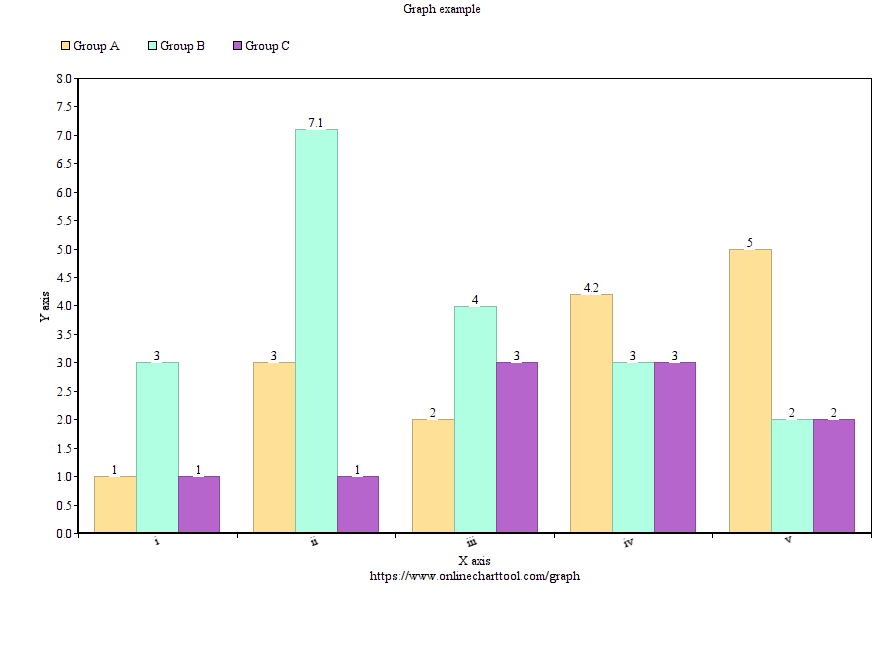
\includegraphics[width=1\textwidth]{img/chart01.png}
            \caption{This is the caption!}
        \end{figure}

        \paragraph*{} This is a continuation of the subsection. Used \url{https://www.sharelatex.com/learn/Inserting_Images} as reference for this subsection.

    \subsection{Creating tables}
        \paragraph*{} Using \url{https://www.sharelatex.com/learn/Tables} as reference on this subsection.

        \paragraph*{} The table \ref{table:1} is an example of referenced \LaTeX elements.
         
        \begin{table}[h!]
            \centering
            \label{table:1}
            \begin{tabular}{||c c c c||} 
                \hline
                Col1 & Col2 & Col2 & Col3 \\ [0.5ex] 
                \hline\hline
                1 & 6 & 87837 & 787 \\ 
                2 & 7 & 78 & 5415 \\
                3 & 545 & 778 & 7507 \\
                4 & 545 & 18744 & 7560 \\
                5 & 88 & 788 & 6344 \\ [1ex] 
                \hline
            \end{tabular}
            \caption{Table to test captions and labels}
        \end{table}

    \subsubsection{Subsection with a label}
    \label{ssub:sdsd}
        \paragraph*{} \lipsum[5]

\section{Section with subsections plus subsubsection}
    \subsection{Subsection}
        \paragraph*{} \lipsum[1]
        \subsubsection{Subsubsection}
            \paragraph*{} \lipsum[5]

\section{Creating references}
    \subsection{Books} \label{books}
        \paragraph*{} Making a reference to the book\cite{book01}.

    \subsection{Footnote}
        \paragraph*{} We have a normal footnote \footnote{Works like a charm.} here.

    \subsection{Cross referencing section}
        \paragraph*{} Here we cross reference section \ref{books}.

\section{Listing}
    \begin{itemize}
        \item Zach Scrivena - \url{https://github.com/zachscrivena/simple-thesis-dissertation}
        \item Sharelatex - \url{https://www.sharelatex.com/}
    \end{itemize}

% ====================================
% BIBLIOGRAPHY and REFERENCES.
% ====================================
\newpage
\nocite{*} % Adds all references available
\setstretch{1}
    \phantomsection % necessary for the linking of this section
    %\addcontentsline{toc}{section}{Bibliografia}

    \printbibliography[heading=bibintoc,type=online,title={Bibliografia}]
    \printbibliography[heading=subbibintoc,type=article,title={Articles only}]
    \printbibliography[heading=subbibintoc,type=book,title={Books only}]
\newpage

\end{document}